% This is "sig-alternate.tex" V2.0 May 2012
% This file should be compiled with V2.5 of "sig-alternate.cls" May 2012
%
% This example file demonstrates the use of the 'sig-alternate.cls'
% V2.5 LaTeX2e document class file. It is for those submitting
% articles to ACM Conference Proceedings WHO DO NOT WISH TO
% STRICTLY ADHERE TO THE SIGS (PUBS-BOARD-ENDORSED) STYLE.
% The 'sig-alternate.cls' file will produce a similar-looking,
% albeit, 'tighter' paper resulting in, invariably, fewer pages.
%
% ----------------------------------------------------------------------------------------------------------------
% This .tex file (and associated .cls V2.5) produces:
%       1) The Permission Statement
%       2) The Conference (location) Info information
%       3) The Copyright Line with ACM data
%       4) NO page numbers
%
% as against the acm_proc_article-sp.cls file which
% DOES NOT produce 1) thru' 3) above.
%
% Using 'sig-alternate.cls' you have control, however, from within
% the source .tex file, over both the CopyrightYear
% (defaulted to 200X) and the ACM Copyright Data
% (defaulted to X-XXXXX-XX-X/XX/XX).
% e.g.
% \CopyrightYear{2007} will cause 2007 to appear in the copyright line.
% \crdata{0-12345-67-8/90/12} will cause 0-12345-67-8/90/12 to appear in the copyright line.
%
% ---------------------------------------------------------------------------------------------------------------
% This .tex source is an example which *does* use
% the .bib file (from which the .bbl file % is produced).
% REMEMBER HOWEVER: After having produced the .bbl file,
% and prior to final submission, you *NEED* to 'insert'
% your .bbl file into your source .tex file so as to provide
% ONE 'self-contained' source file.
%
% ================= IF YOU HAVE QUESTIONS =======================
% Questions regarding the SIGS styles, SIGS policies and
% procedures, Conferences etc. should be sent to
% Adrienne Griscti (griscti@acm.org)
%
% Technical questions _only_ to
% Gerald Murray (murray@hq.acm.org)
% ===============================================================
%
% For tracking purposes - this is V2.0 - May 2012

\documentclass{sig-alternate}
\usepackage{multirow}
\begin{document}
%
% --- Author Metadata here ---
\conferenceinfo{OCL}{'12, September 30 2012, Innsbruck, Austria}
\CopyrightYear{2012} % Allows default copyright year (20XX) to be over-ridden - IF NEED BE.
\crdata{978-1-4503-1799-3/12/09}  % Allows default copyright data (0-89791-88-6/97/05) to be over-ridden - IF NEED BE.
% --- End of Metadata ---

\title{An extensible OCL Virtual Machine and Code Generator}

%
% You need the command \numberofauthors to handle the 'placement
% and alignment' of the authors beneath the title.
%
% For aesthetic reasons, we recommend 'three authors at a time'
% i.e. three 'name/affiliation blocks' be placed beneath the title.
%
% NOTE: You are NOT restricted in how many 'rows' of
% "name/affiliations" may appear. We just ask that you restrict
% the number of 'columns' to three.
%
% Because of the available 'opening page real-estate'
% we ask you to refrain from putting more than six authors
% (two rows with three columns) beneath the article title.
% More than six makes the first-page appear very cluttered indeed.
%
% Use the \alignauthor commands to handle the names
% and affiliations for an 'aesthetic maximum' of six authors.
% Add names, affiliations, addresses for
% the seventh etc. author(s) as the argument for the
% \additionalauthors command.
% These 'additional authors' will be output/set for you
% without further effort on your part as the last section in
% the body of your article BEFORE References or any Appendices.

\numberofauthors{1}
\author{
% You can go ahead and credit any number of authors here,
% e.g. one 'row of three' or two rows (consisting of one row of three
% and a second row of one, two or three).
%
% The command \alignauthor (no curly braces needed) should
% precede each author name, affiliation/snail-mail address and
% e-mail address. Additionally, tag each line of
% affiliation/address with \affaddr, and tag the
% e-mail address with \email.
%
% 1st. author
\alignauthor
E.D.Willink\\
       \affaddr{Eclipse Modeling Project}\\
       \email{ed@willink.me.uk}
}

\maketitle
\begin{abstract}
The Object Constraint Language (OCL) is a specification language that is also executable
and so a variety of OCL execution capabilities have evolved. Some are interpreted while
others use a code generator for an implementation language such as Java. The mapping
of much of OCL to Java is obvious and so many implementations pursue the obvious approach
but then find that the approach can only support an OCL subset.

In this paper we revisit OCL evaluation. We first establish a simple uniform execution framework
that applies to the whole of OCL. We call this an OCL Virtual Machine.
We then identify how optimizations can bridge the gap between
the uniform framework and how applicability predicates can determine when the optimization can
be applied without needing to resort to a subset OCL. We finally identify how this uniform
framework is extensible to OCL-based languages such as QVT.
\end{abstract}

% A category with the (minimum) three required fields
%\category{H.4}{Information Systems Applications}{Miscellaneous}
%A category including the fourth, optional field follows...
%\category{D.2.8}{Software Engineering}{Metrics}[complexity measures, performance measures]
\category{D.3.4}{Processors}{Run-time environments, Code generation}

%\terms{Theory}

%\keywords{ACM proceedings, \LaTeX, text tagging} % NOT required for Proceedings

\section{Introduction}
It is nearly 20 years since OCL first emerged at IBM as an evolution from Syntropy, and nearly 10 years since the OCL 2.0 specification was drafted\cite{OCL-2.0-draft}. OCL is critical to the specification of UML and since no clear alternative to UML or OCL has emerged, why is OCL uptake so limited?

Perhaps OCL enthusiasts need to be honest and look hard at why OCL doesn't work today.
Then it may be possible to realize the tremendous promise for the future and to exploit the many
demonstrations of the power of OCL formality at research institutions.

\subsection{Quality}

The main official examples of OCL come from the UML 2.4.1\cite{UML-2.4.1-Super} and OCL 2.3.1\cite{OCL-2.3.1} specifications. Analysis\cite{UML-inconsistent} of the UML Superstructure specification has identified that over 50\% of the 235 Well-Formedness Rules (WFR) have basic syntactic or semantic errors
that any competent OCL tooling should detect. The `correctness' of the OCL in UML 2.4.1 is almost unchanged
since UML 2.0.

If the WFRs are so semantically incorrect, what chance is there that they are functionally useful?

Can we expect the wider software community to take OCL seriously when its most obvious exposition is so poor?

The UML 2.5 specification is now `complete' and undergoing review. The specification is a major simplification. It
reorganizes the previous layers of merge-able concepts in the Superstructure and Infrastructure specifications into
a single specification of the merged concepts; this is a tremendous improvement and is supported by the use of
model-driven auto-generation of the specification from normative models. With high quality models in place, attention has
turned to the OCL embedded within them. Eclipse OCL\cite{MDT/OCL} tooling was used to remove 74 syntax errors and correct one or more semantic errors in 250 distinct text regions. Further errors were corrected as missing OCL constraints were added and Diagram Interchange introduced.
For the most part, the use of Eclipse OCL in the form of IBM's RSA, allowed authors to correct their own errors directly.

The UML 2.5 embedded OCL is therefore potentially free of syntax and semantic errors, but is it functionally useful?

The constraints are often the primary specification so there is a little to check them against apart from common sense.
Some errors may be detected by analysis tools that look for redundancy and contradiction. But in practice, we need to
execute them and so discover constraints that are too strong and which reject useful models. Uncovering constraints
that are missing or too weak may depend on alert reviewers, users and toolsmiths.

In this paper we discuss work in Eclipse OCL to make the OCL embedded within the UML and OCL specifications usefully
executable. On the one hand this facilitates the empirical discovery of the meaningless or over-strong WFRs, and on the other avoids the need for a manual transcription of the WFRs to an implementation language. It also avoids the associated transcription errors. In Section \ref{VM now} we describe the features of the OCL VM that supports this, and in Section \ref{VM future} we discuss optimization to give dramatic performance improvements. 

\subsection{Speed}
Attempting to use OCL in earnest encounters another credibility gap. OCL execution is often slow, despite the very favorable showing of Eclipse OCL in comparison with other technologies reported in Slide 11 of \cite{Rath-Queries}.

In Eclipse OCL, this is because execution has used an interpreter; directly on Ecore for many years, and recently
on a UML-aligned pivot representation. Table \ref{Evaluator performance} shows the relative performance using the simplest benchmark from \cite{Rath-Queries} for which the minimal Java code is just
\begin{verbatim}        return this.feature <= 0\end{verbatim}
 evaluated on a set of 12800 model elements.
A preliminary code generator was introduced in the Juno release and this gives a 3-fold
improvement. Manual execution of plausible optimizations of the auto-generated code suggests that the minimal code is obtainable and so in total there is perhaps a 500-fold improvement available. 

\begin{table}
\centering
\caption{Eclipse OCL Evaluation Assessment}\label{Evaluator performance}
\begin{tabular}{|c|c|c|} \hline
Approach&Release&Performance\\ \hline
Direct Ecore interpreter & ..., Juno & 72 ms\\ \hline
Pivot Value interpreter & Indigo, Juno & 88 ms \\ \hline
Pivot Value code gen & Juno & 22 ms \\ \hline
`Optimized' code gen & manual & 0.13 ms \\ \hline
\end{tabular}
\end{table}

Naive validation of large UML models is slow and any loss of performance approaching 500-fold is
obviously unacceptable for everyday tooling. The evaluation performance of Dresden OCL was reported as four times slower than Eclipse OCL, so the problem is not unique to Eclipse OCL; better code generation  is available in research tools, but
accurate fast evaluation has not made it into the mainstream tools.

\subsection{Basic Code Generation}

OCL has many superficial similarities to Java and so it is intuitively attractive to just translate OCL into Java and many authors have done this. Unfortunately OCL is not the same as Java and the intuitive translation only works easily for a Java-like OCL subset.

Some of the problems that a full-functionality OCL evaluator must accommodate are:
\begin{itemize}
\item An Integer has no upper bound; Java's int and long have upper bounds.
\item An UnlimitedNatural is-a Integer which is-a Real; Java numeric classes are unrelated.
\item UnlimitedNatural values have an unlimited value
\item Datatype equality is determined by value and so 4 is equal to 4.0; Java numeric objects are unrelated.
\item Set(T) entry uniqueness is determined by datatype equality; Java object equality is different.
\item All types conform to OclAny
\item Collections can be nested and can contain null values
\item Null values may participate in computations and the OclVoid type conforms to all types
\item Invalid values may participate in computations but may not be used in collections
\item Operations may be overloaded
\item Additional features may be added by a Complete OCL document
\item oclType() may be a gateway to reflective functionality
\item allInstances() requires access to a global model view 
\item The specification lacks precision in some critical areas
\end{itemize}

\section{OCL Virtual Machine}\label{VM now}

\begin{figure}
  \begin{center}
    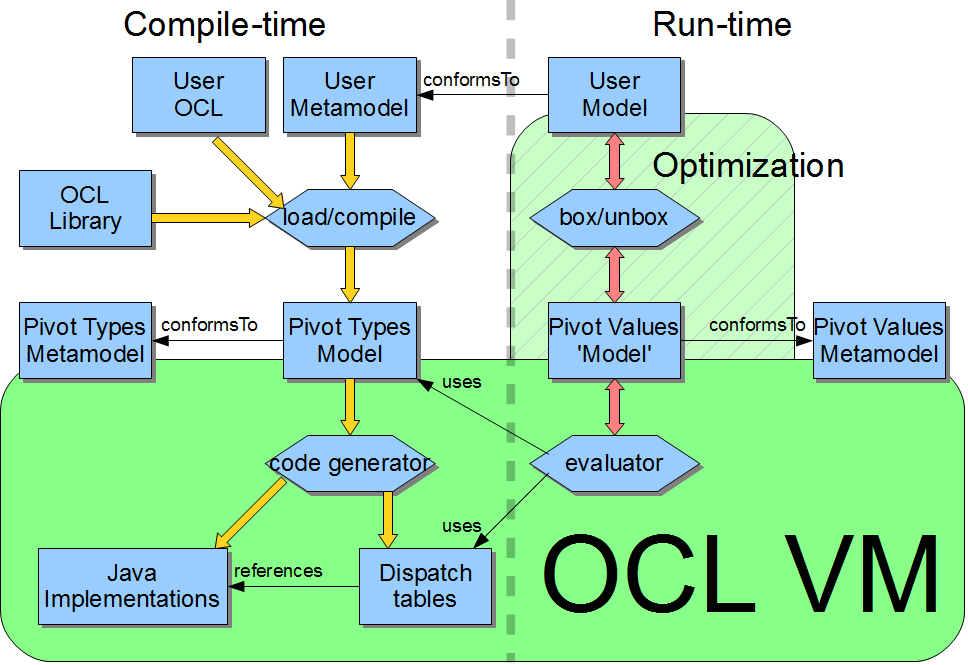
\includegraphics[width=3.25in]{OCL2012OCLVM.png}
  \end{center}
  \caption{The OCL VM.}
  \label{fig:OCLVM}
\end{figure}

Figure \ref{fig:OCLVM} shows the context of the OCL VM. On the left hand side we have the compile-time activities in which
user meta-models, user OCL and OCL libraries are loaded, normalized and compiled to give the Pivot Type representation
of the structural models and the Abstract Syntax Tree (AST) of each OCL expression.
On the right hand side we have the run-time activities in which user models are accessed by the evaluator to perform the required computations. In this section, we describe the various elements of the OCL VM that give a simple predictable full functionality framework. In the next section, we consider optimizations to avoid the overheads of boxing and unboxing model elements
and speed-ups for the generated Java implementations.
  
The classes of the AST such as IfExp and OperationCallExp have distinct but relatively simple semantics, so that it is not difficult for a tree walking evaluator to start at an expression root node and use the appropriate
node-class-specific semantics to visit each node in the tree to compute the value of the OCL expression. 
%Since OCL is side effect free it is even permissible for parallel execution to visit different parts of the tree concurrently.

We will examine this evaluation in a little more detail to see how the basic computation elements of values and types
are used by an operation implementation associated with each AST node.

\subsection{Pivot Value System}

Evaluation requires values to compute with and computation is easier when the values are polymorphic and observe OCL semantics. Neither of these is a characteristic of an implementation language such as Java in which 
\begin{itemize}
\item Boolean, BigInteger, String and Set share no useful inheritance
\item Object rather than DataType equality applies to numbers 
\item Unbounded Numerics are costly 
\end{itemize}

We therefore take the hint from Clause 10.2 of the OCL specification and use polymorphic values.
A polymorphic Value system can have a family of IntegerValue implementations so that
 \begin{itemize}
\item IntIntegerValueImpl wraps a 32 bit java.lang.int
\item LongIntegerValueImpl wraps a 64 bit java.lang.long 
\item BigIntegerValueImpl wraps java.number.BigDecimal \linebreak for unbounded support.
\end{itemize}
IntIntegerValueImpl is almost identical to java.lang.Integer, except that 
\begin{itemize}
\item numeric overflow is detected to promote growth to a LongIntegerValueImpl
\item equality is re-implemented so that same-valued Real and Integer values are equal.
\end{itemize}
For typical 32 bit usage, the performance penalty of using IntIntegerValueImpl rather than java.lang.Integer is small, and where necessary the unbounded OCL requirements are supported.

The Value types specified by the OCL specification and those used in the OCL VM are shown in the second and third columns of Table \ref{Values+Types}. The differences show the need for a certain amount of remedial action
\begin{itemize}
\item Boolean/Real/Integer/Invalid/OrderedSet Values are defined
\item Bag/Sequence/EnumerationLiteral Values are spelled consistently 
\item Type-valued expressions are are supported.
\end{itemize}

Use of types as values is implicit in OCL expressions such as \verb|oclIsKindOf(SomeType)| but left rather vague in the specification. A practical system must recognize that types can be values and that their types can be templated. Thus a modeled
library element declaration\cite{OCL-stdlib} might be:
\begin{verbatim}
operation oclAsType<TT>(type : Metaclass<TT>) : TT
\end{verbatim}
%This enables the type system to propagate the known argument type to the result.

\begin{table*}\label{Values+Types}
\centering
\caption{OCL (Pivot) Values and Types }
\begin{tabular}{|c|c|c|c|c|} \hline
Type Name&OCL 2.3.1 Value&OCLVM Value&OCL 2.3.1 Type&OCLVM Type\\ \hline\hline
OclAny &\multicolumn{2}{|c|}{Value}&\multicolumn{2}{|c|}{AnyType}\\ \hline\hline
Boolean & ? & BooleanValue & BooleanType & PrimitiveType \\ \hline
String & \multicolumn{2}{|c|}{StringValue} & \multicolumn{2}{|c|}{PrimitiveType} \\ \hline
Real & ? & RealValue & \multicolumn{2}{|c|}{PrimitiveType} \\ \hline
Integer & \multirow{2}{*}{?} & IntegerValue & \multicolumn{2}{|c|}{\multirow{2}{*}{PrimitiveType}} \\ 
UnlimitedNatural &  & UnlimitedValue & & \\ \hline
OclVoid & OclVoidValue & NullValue & \multicolumn{2}{|c|}{VoidType} \\ \hline
OclInvalid & ? & InvalidValue & \multicolumn{2}{|c|}{InvalidType} \\ \hline\hline
Collection &  \multicolumn{2}{|c|}{CollectionValue} &  \multicolumn{2}{|c|}{CollectionType} \\ \hline
Bag & BagTypeValue & BagValue & \multicolumn{2}{|c|}{BagType} \\ \hline
OrderedSet & ? & OrderedSetValue & \multicolumn{2}{|c|}{ OrderedSetType} \\ \hline
Sequence & SequenceTypeValue & SequenceValue & \multicolumn{2}{|c|}{SequenceType} \\  \hline
Set & SetTypeValue & SetValue & \multicolumn{2}{|c|}{SetType} \\ \hline \hline
Tuple & \multicolumn{2}{|c|}{TupleValue} & \multicolumn{2}{|c|}{TupleType} \\ \hline
EnumerationLiteral & EnumValue & EnumerationLiteralValue & ? & Type \\ \hline
Object & \multicolumn{2}{|c|}{ObjectValue} & ? & OclElement \\ \hline
Type & ? & TypeValue & ? & OclType \\ \hline
Lamda &  &  & ? & LambdaType \\ \hline
\end{tabular}
\end{table*}

\subsection{Pivot Type System}

Values of course have types, and with a polymorphic value system, the type is available internally as \verb|Value.getType()| which provides the underlying support for a fully reflective  \verb|oclType()|.

The Type types specified by the OCL specification and those used in the UML-aligned OCL VM\cite{OCL-UML} are shown in the fourth and fifth columns of Table \ref{Values+Types}.

For the basic data types, the only change is the removal of BooleanType which becomes redundant if a static (metaclass) method of Boolean rather than an instance method of a metaclass is used to model \verb|Boolean.allInstances()|.

For object types, the specification is vague as to how UML-defined types conform to OclAny and what functionality they inherit as a result. The OclElement type that conforms to OclAny is introduced in the Pivot type system as the superclass of all UML-defined types that lack an explicit superclass. OclElement provides added functionality such as allInstances() and oclContainer(). OclType imposes further standard functionality on all types.

LambdaTypes are implicit in OCL as the type of an iterator body\cite{OCL-stdlib}. A corresponding LambdaValue unifying ExpressionInOCL may be appropriate for more flexible higher order support.

Finally ObjectValue provides the polymorphic pivot to a practical representation such as an EObject by a derived EObjectValueImpl. 

\subsection{Variables and Environment}

Typed Variables (or Parameters) are introduced by the invocation context, let-expressions and iterator-expressions. The OCL specification defines a moderately complex Environment to maintain name value bindings. These are resolved at compile time
so that AST nodes have properties such as \verb|VariableExp.referredVariable| for an intermediate value or \verb|PropertyCallExp.referredProperty| for a model access. There are two exceptions to this.

The OCL specification does not model iterations and so there is no  \verb|IteratorExp.referredIteration|. Iterations are resolved by a run-time name lookup. The OCL VM models an \verb|Iteration| as an extension of \verb|Operation| and so can exploit an \verb|IteratorExp.referredIteration|\cite{OCL-UML}.

Operations (and iterations)  can be overloaded, although the OCL specification fails to define a dynamic dispatch algorithm. The OCL VM dynamic dispatch support is described in \ref{DispatchTables}.

\subsection{Operations}

With values and types, we just need some operations to perform computations. Do we need anything else?

\subsubsection{If}

An if-expression evaluates only one of its \verb|then| or \verb|else| arguments, so an if-expression must be handled separately from operations.

\subsubsection{Literal}

A literal expression could be regarded as a zero argument static operation of OclAny, but a literal is easily optimized so there is little point changing the distinct treatment defined by the OCL specification.

\subsubsection{Model Access}

\verb|AssociationClassCallExp| and \verb|PropertyCallExp| nodes provide the interaction between user models and the OCL evaluation. The various accesses can be modeled as operation on a host \verb|ObjectValue|. The OCL VM therefore augments each property in the metamodel with an implementation appropriate to the composition, multiplicity or navigability characteristics of the property. This migrates some computation from run-time to compile-time.

\subsubsection{Operation Bodies}

Once an operation has been determined, an executable implementation of the operation body must be located to evaluate the operation. The compiler therefore annotates each operation (and iteration) in a similar way to properties with an appropriate implementation of the operation.

\subsection{Dispatch Tables}\label{DispatchTables}

Dynamic dispatch requires selection of the operation implementation appropriate to the actual source type of an operation. If such a selection is made on a typical metamodel representation, it may be necessary to perform a 6-dimensional search
\begin{itemize}
\item Each of the immediate superclasses 
\item Each of the inherited superclasses
\item Each of the operations to match the name
\item Each of the parameters to match the name
\item Each of the parameter type immediate superclasses for conformance
\item Each of the parameter type inherited superclasses for conformance.
\end{itemize}
This can be very expensive in deep inheritance hierarchies and often redundant since there may be no overload to resolve.

The OCL VM therefore prepares dispatch tables for which the static referredOperation provides an integer
operation signature index and inheritance depth reducing the problem to 1-dimensional 
\begin{itemize}
\item Each of the same-depth superclasses 
\end{itemize}

In practice even deep inheritance trees are relatively narrow so the search usually involves a simple indexed lookup in a single class. Only rarely is it necessary to examine two or three alternatives.

The dispatch tables also support improved speed for type conformance checks underlying \verb|oclIsKindOf()| and reflective operations such as \verb|oclType().ownedOperations()|.

\section{Code Generator}\label{VM future}

The Juno release of the Eclipse OCL Examples and Editors includes an experimental release of the OCL VM support,
in which the code generator is integrated with the EMF model generator. If the OCL preference page option to use the code generator is enabled, EMF generation then provides the OCL VM dispatch tables and implementations automatically.

The Juno release pursues the naive approach of serializing the OCL AST as Java code that sequences the
dynamic dispatch of an operation for each operation-like AST node. The resulting code is simple and supports the
full OCL semantics\footnote{ oclIsNew(), @pre, States and Messages are to-be-done}. The three-fold speed up compared to the interpreted approach is useful but not spectacular. Additionally, the run-time compilation costs are eliminated since the OCL parsing now occurs at compile-time. 

The Juno code generator uses Acceleo Model to Text templates to perform a direct AST model to Java text translation. A class comprising a single polymorphic function for each implementation. The function body contains two text regions. 

The first text region provides a constant and variable declarations. Common Subexpression Elimination is achieved by the simple strategy of pruning duplicate text lines. 

The second text region sequences the implementation calls from an AST tree walk. Since everything is an implementation call and there is no inlining yet, there are no operation-specific patterns as used by other authors.

\subsection{Optimizations}

With a full-functionality VM in place, it is now possible to look at optimizations that perform M2M rewrites of the OCL AST before performing the final M2T code generation to a preferred target language.

Initial manual experiments suggest that a further 100-fold speed improvement is available by:
\begin{itemize}
\item Directly accessing EMF properties as getXX(), rather than eGet(XX) 
\item Directly dispatching operations for which dynamic dispatch is redundant
\item Inlining operations that are directly dispatched
\item Unboxing Pivot Values to use the underlying Java values or EObjects directly
\item Using an Unboxed operation call in the VM 
\item Directly accessing EMF object fields and bypassing getXXX().
\item Performing a direct Collection mutation to re-use a no-longer-used Collection 
\end{itemize}

Each of the above optimizations has associated guard conditions, so for instance an \verb|IntegerValue| can only be unboxed to an \verb|int| if the dynamic range can be analyzed and found compatible with 32 bits. Unfortunately UML does not naturally support specification of value bounds, so opportunities for unboxing are limited to discovering that the source value is 32 bits and propagating until arithmetic is performed.

Similarly the absence of invalid and null values must be ascertained to allow the associated polymorphism to be discarded.

The progressive application of optimizations to a valid AST with full OCL functionality offers the prospect of retaining full-functional validity after optimizations. This is difficult to achieve when a direct single stage pattern pasting approach to code generation is taken. 

\subsection{Beyond OCL}

Efficient evaluation of OCL is useful, but increasingly OCL is now used within extended contexts such as QVT\cite{QVT-1.1} or MOFM2T\cite{MOFM2T}.
These languages define an extended AST and so in principle are amenable to the same tree-walking evaluation as the basic OCL AST. In practice, and in particular for QVT Relations, substantial strategic planning will be needed prior to evaluation. Nonetheless the same basic interpreter can support naive evaluation and the code generator can be extended to the extended AST.

QVT Operational introduces an Imperative OCL extension that clearly violates the side effect free characteristics of OCL.
This requires a two level approach with an overall structure that sequences side effect free
OCL sections.  

\section{Related Work}

Many authors have provided a partial OCL code generator demonstrating good characteristics aligned with some research goal. Omission of OCL facilities such as oclIsNew(), @pre,  allInstances(), States, Messages and even Tuples and opposites is common, but in many cases this just represents a pragmatic reduction of scope to facilitate research; these omissions can be rectified by a little more work. Failure to address unbounded numerics, numeric equality, null/invalid propagation, nested Collections and oclType() is a more fundamental challenge to some of the approaches. 

Wilke\cite{Dresden/JavaCG} describes a reworked  Java generator for Dresden OCL based on parameterized fragments.
AspectJ is used to support model access in Java models. However many Java types are used directly and so functionality is limited to Java-like semantics for numeric range and equality.

Heidenreich\cite{QueryCode} describes a Dresden OCL generator for SQL based on identifying typical patterns of database usage. It is not clear that this is able to handle arbitrary OCL or OCL that fails to exhibit SQL-like characteristics.

Egea\cite{MySQL4OCL} describes a MySQL generator to avoid the heavy overhead of loading a large model into an OCL tool. Stored procedures are used to realize the iterations that are common to many typical applications. The procedures are then executed within an SQL database. This is an interesting deployment option but does not help with full-functionality OCL code generation.

Shidqie\cite{Shidqie} introduces Imperative Ecore as an intermediate model to separate OCL restructuring and Java formatting concerns, but ignores non-Java-like aspects such as unbounded numbers.

Moiseev\cite{rodion-models2009} takes a more progressive transformational approach realized as rewrites in Maude. This is clearly beneficial when supporting multiple target languages, unfortunately it ignores the awkward aspects of OCL.

Mezei\cite{OCL-relocation} relocates and caches OCL evaluations to reduce navigation costs.

Efficient code is one important aspect of OCL execution. Efficient scheduling is an equally important
but largely orthogonal issue. 
Cabot\cite{Constraint-Survey} provides a review of the disappointing scheduling
support in many tools that support Constraint evaluation.
Eclipse OCL was overlooked in the review. Eclipse OCL inherits the default EMF capability
to perform a total validation. Eclipse OCL has an Impact Analyzer that supports selective re-evaluation.

The need for variability in both the type and value system was recognized by Wilke\cite{Variability}. The pivot Value
and Type systems correspond to the variation points but normalize the external view to support a uniform OCL engine rather than adapting the engine to the external.

The very useful concept of a pivot\cite{Pivot} model was introduced by Dresden OCL.

\section{Conclusions}
We have identified the poor quality of official OCL expositions and the poor speed of accurate OCL
evaluation as problems for OCL credibility in the wider software community. The imminent step
change in quality with the UML 2.5 WFRs provides a further stimulus to tackle fast accurate evaluation.

We have noted the semantic differences between OCL and Java and the consequent difficulties of a direct
translation for more than a Java-like OCL subset.

In contrast we have noted that the OCL AST is very amenable to a tree-walking evaluation, and described how
a uniform polymorphic Pivot Value system and an associated Pivot Type system can support evaluation using
an appropriate node-specific implementation.

The OCL VM's dispatch tables, which are automatically generated during EMF model generation
have been outlined and shown to reduce a potentially six dimensional search for operation
dynamic dispatch to barely one dimensional.

The experimental implementation of the above gives only a three-fold speed-up compared to interpretation. Manual
experiments of model-to-model transformations that optimize the OCL AST have demonstrated that there is a 
500-fold improvement available.

Extension of the OCL VM to support OCL-based languages should be possible.
%\end{document}  % This is where a 'short' article might terminate

%
% The following two commands are all you need in the
% initial runs of your .tex file to
% produce the bibliography for the citations in your paper.
\bibliographystyle{abbrv}
\bibliography{OCL2012OCLVM}
% You must have a proper ".bib" file
%  and remember to run:
% latex bibtex latex latex
% to resolve all references
%
% ACM needs 'a single self-contained file'!
%
%\balancecolumns
\balancecolumns
% That's all folks!
\end{document}
